\chapter{Phase Detector Project}
\glsresetall
\label{chapter:phase_detector}

\section{Introduction}

In this lab, you will design the phase detection part of a receiver by implementing a complex FIR filter and a COordinate Rotation DIgital Computer (CORDIC) module. You are going to build a complex FIR filter utilizing four ``real'' FIR filters similar to what you developed in Project 1 (see Chapter \ref{chapter:FIR_Project}).  

The complex FIR filter is used to correlate to a known complex signal.  We use Golay codes which have some great properties related to orthogonality and auto-correlation. This is not important to this lab, but is some really amazing math. I hope you look into it.

The CORDIC function is built from scratch and will likely take a large amount of your time for this assignment. A CORDIC is an efficient method for calculating  trigonometric and hyperbolic functions. CORDIC can do a lot of different functions; we will use it to convert Cartesian coordinates $(x,  y)$ to the polar coordinates $(r, theta)$. 

In the end, you will combine all of these modules into something that is the beginning of a digital communication receiver. The goal is to do simple synchronization and discover the phase of the signal. The output of the CORDIC $(r, theta)$ gives you these results. It is not everything that you need to do, but it is a good start. 

The provided Simulink file gives the transmitter, channel, and receiver. You are building an equivalent receiver in HLS in this project. We used this Simulink project to create the various testbenches for the project.

Finally, you will demonstrate a working system of the complete phase detector using Xilinux on the Zedboard. 

\section{Materials}

The provided folder has a number of subfolders and files corresponding to the different parts of the phase detector.  This contains the documents necessary to build the project. In this folder you will see two folders. One is HLS and other is demo. You will start from HLS folder to design your phase detector using \VHLS.
\begin{itemize} 
\item \texttt{HLS/fir} folder: This folder contains \texttt{*.cpp}, \texttt{*.h}, and script files for a complex FIR filter. The complex is matched filter. You are matching the complex I and Q Golay codes. You can to design the complex FIR filter using your \texttt{fir()} function Project 1. In the \texttt{fir.cpp} file, there are four sub functions \texttt{firI1}, \texttt{firI2}, \texttt{firQ1}, and \texttt{firQ2}. These functions are real FIR filters i.e., the same that you designed in Project 1. You can use your favorite code from Project 1 in these four sub functions. In the complex fir filter, four of these functions are used in the \texttt{fir} function. In that function, you need to connect the four FIR filters \texttt{firI1}, \texttt{firI2}, \texttt{firQ1}, and \texttt{firQ2} to an adder and subtractor to create the complex matched filter. This structure is demonstrated in the Simulink file. 

\item \texttt{HLS/cordic} folder:
\begin{itemize}
\item \texttt{cordiccart2pol.cpp}: The place where you write your synthesizable code. Currently, it only contains the function prototype. 
\item \texttt{cordiccart2pol.h}: Header file with various definitions that may be useful for developing your code.
\item \texttt{cordiccart2pol\_test.cpp}: Testbench
\item \texttt{script.tcl} and \texttt{directive.tcl}: Use this to create your project
\end{itemize}

\item \texttt{HLS/phasedetector} folder: After you design the CORDIC and the complex FIR, you will use them to design the phase detector. 
\begin{itemize}
\item \texttt{fir.cpp}:  Real FIR filter that you designed in Project 1. 
\item \texttt{cordiccart2pol.cpp}: \texttt{cordiccart2pol} function you will design in this project.
\item \texttt{phasedetector.cpp}: Top level skeleton for the phase detector. You use \texttt{fir.cpp} and \texttt{cordiccart2pol.cpp} to design the \texttt{phasedetector} function. 
\item \texttt{phasedetector\_test}: Testbench
\item \texttt{phasedetector.h}: Header file
\item \texttt{script.tcl} and \texttt{directive.tcl}: Use this to create your project
\end{itemize}

\item \texttt{Demo} folder: Demo folder for 11 tap filter
\begin{itemize}
\item \texttt{host.c}: Unfinished host program
\item \texttt{exe\_script.sh}: Execution script
\item \texttt{plot\_script.p}: Plotting script
\item \texttt{input\_i.dat}:Input I signal
\item \texttt{input\_q.data}: Input Q signal

\end{itemize}
\end{itemize}

\section{Tasks}

\begin{figure}
\centering
%\includesvg{images/matrix_vector_sequential}
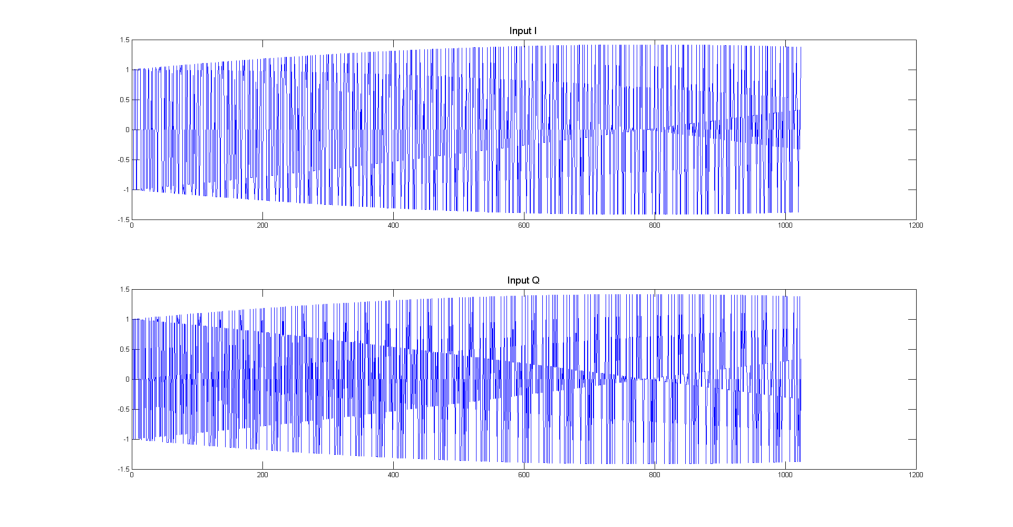
\includegraphics[width=6in]{images/IQ}
\caption{Input I and Q values to your complex FIR filter.} \label{fig:IQ}
\end{figure}

In this project, you will build a phase detector to process the given I and Q signals shown in Figure \ref{fig:IQ}. The final goal is to implement this phase detector on the Zedboard. To achieve this goal, you will need to finish the following 
tasks:
\begin{enumerate}
\item Implement the complex matched filter and verify it with the given testbench. This matched filter consists of four FIR filter modules which are similar to the ones in your Project 1. For the purpose of debugging, if you plot the outputs of this step, you should expect the waveforms as shown in Figure \ref{fig:XY}.
\item Implement the CORDIC HLS code and verify it with the given testbench.
\item Connect the complex matched filter and CORDIC modules to implement the receiver. Verify this overall design with the given testbench. For the purpose of debugging, if you plot the outputs of this step, you should expect the waveforms as shown in the figure below.
\item Implement the receiver design on the Zedboard. This process is similar to the demo in your Project 1. But this time, we will generate the bit file using Vivado instead of ISE. Please read the ``Hints'' section for some tips about this. The expected output is as shown in Figure \ref{fig:phase_detector_demo}.
\end{enumerate}

\begin{figure}
\centering
%\includesvg{images/matrix_vector_sequential}
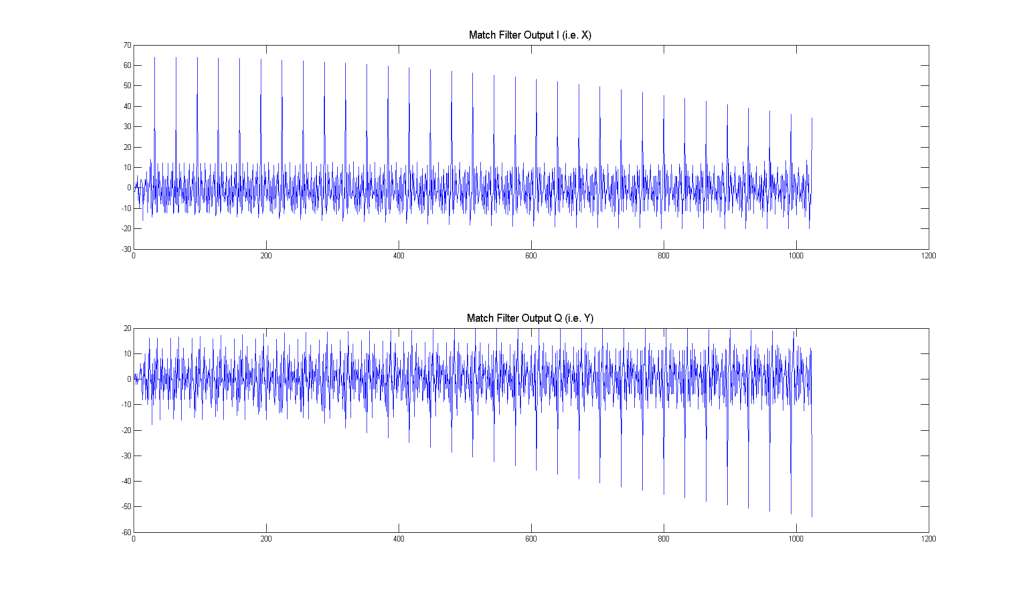
\includegraphics[width=6in]{images/XY}
\caption{Output values from the complex FIR filter corresponding to the inputs from Figure \ref{fig:IQ}.}
\label{fig:XY}
\end{figure}

\begin{figure}
\centering
%\includesvg{images/matrix_vector_sequential}
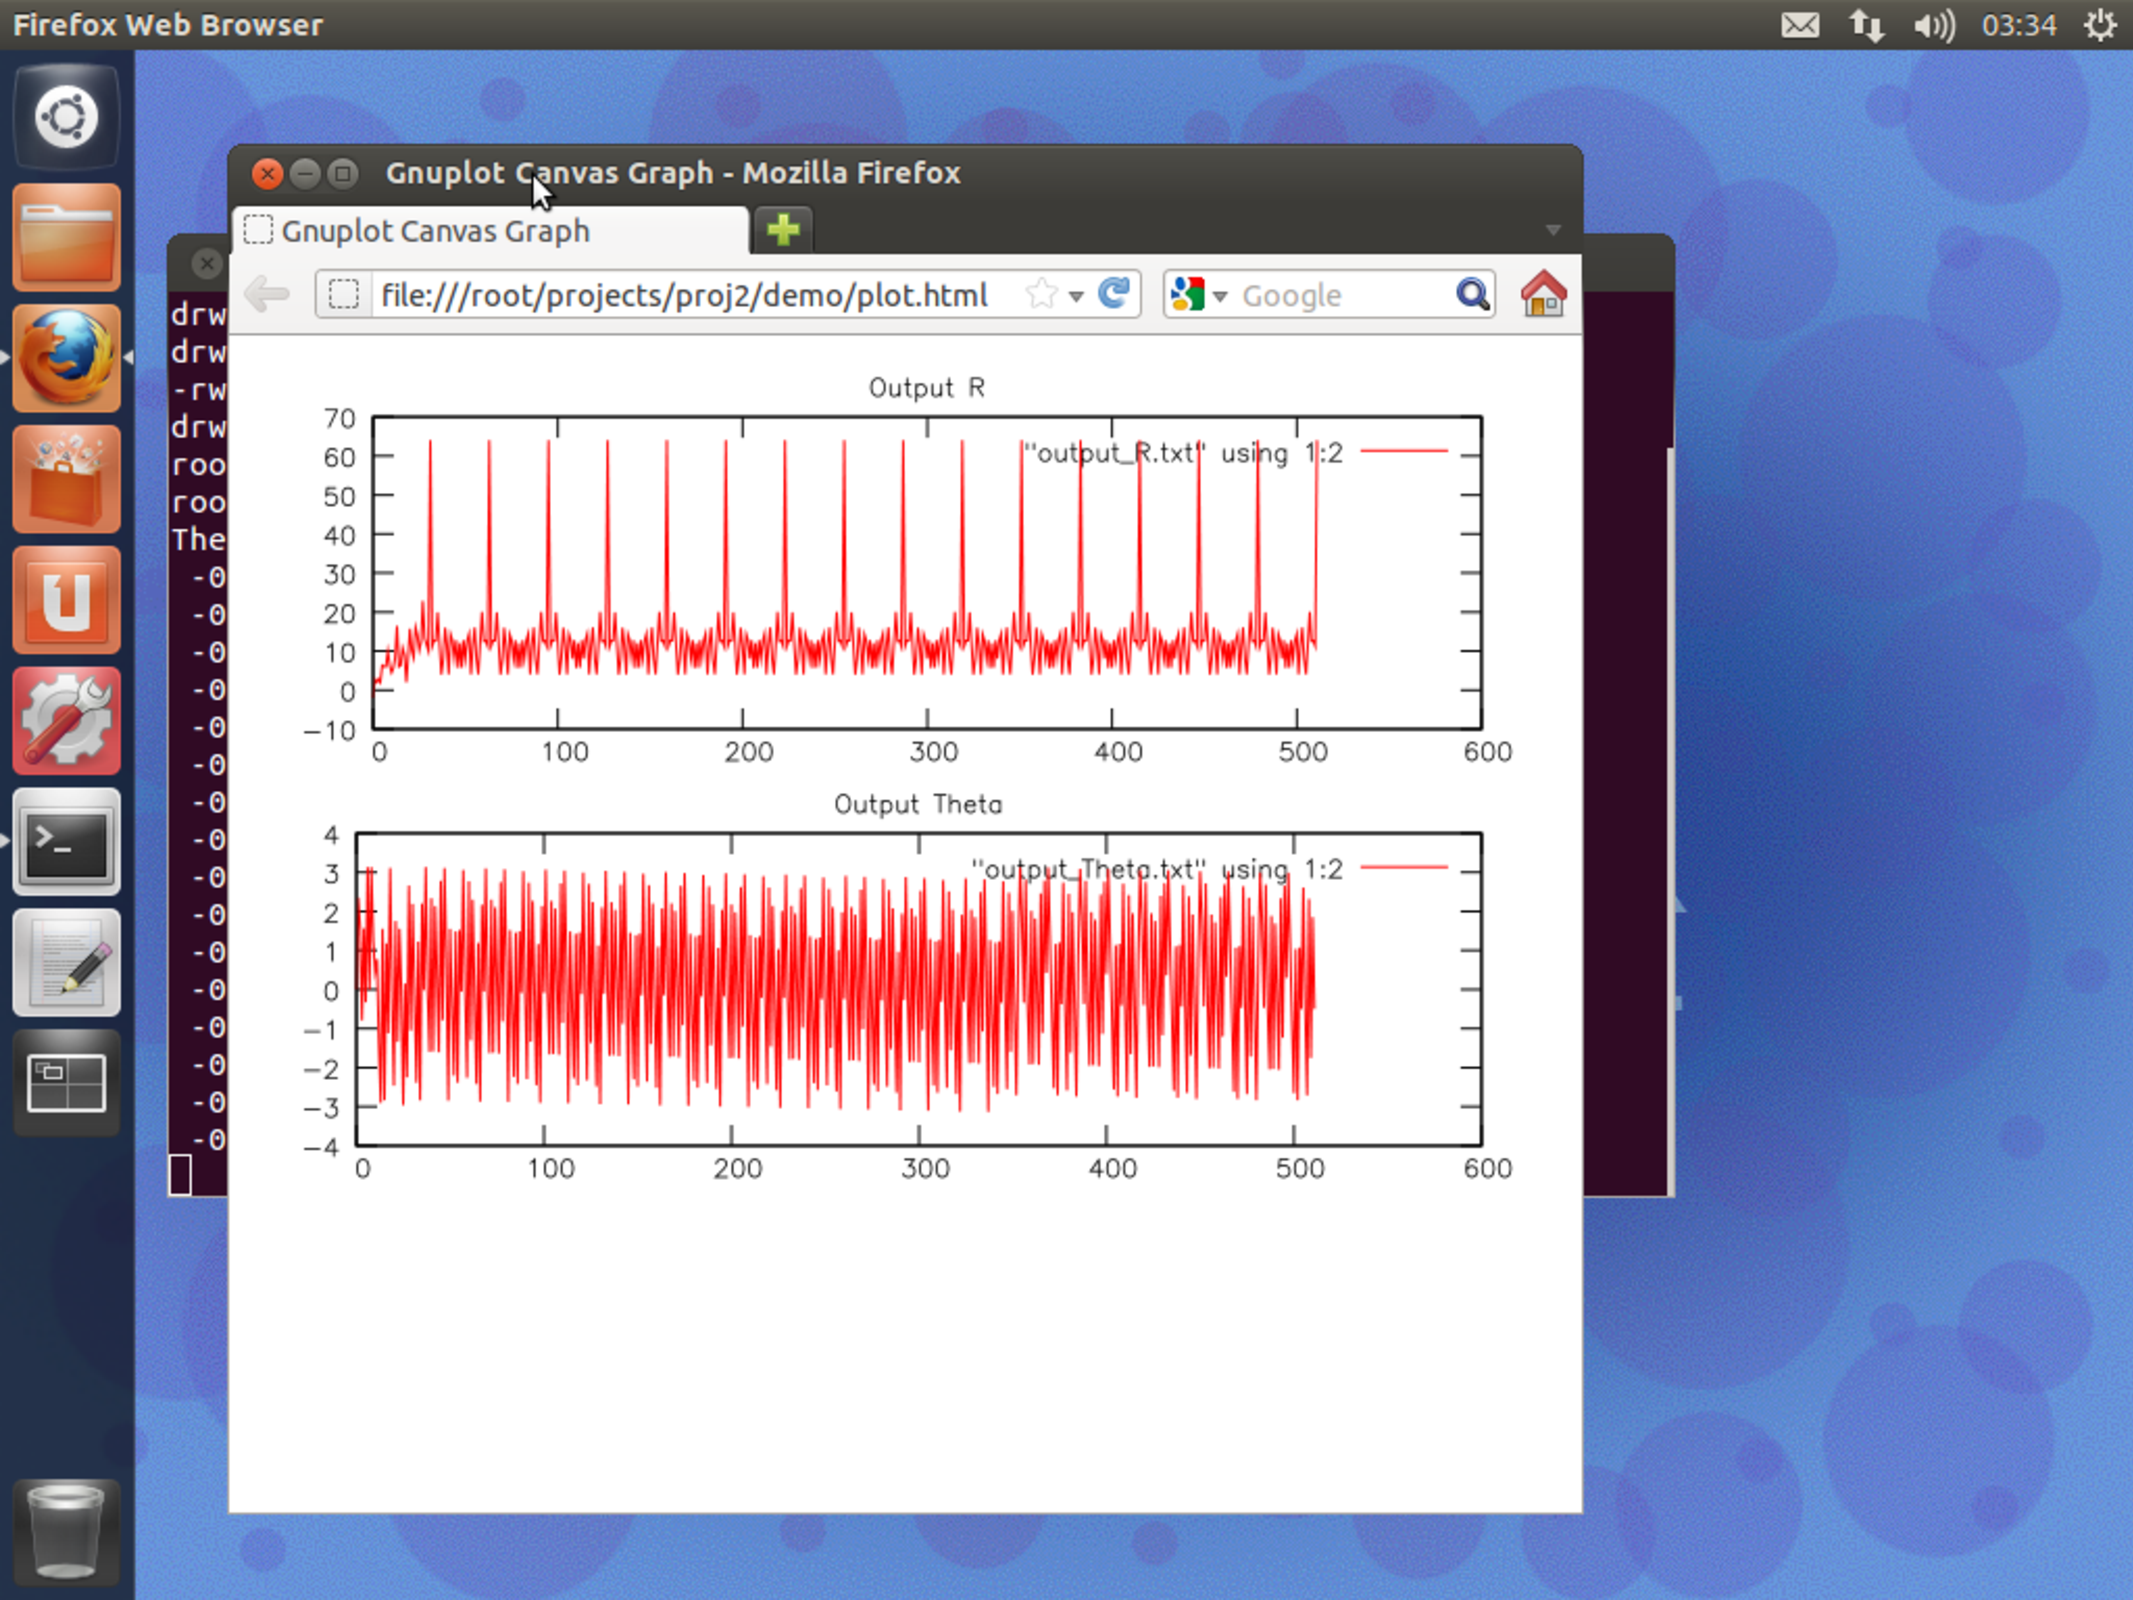
\includegraphics[width=6in]{images/phase_detector_demo}
\caption{Example output plot for the phase detector demo.}
\label{fig:phase_detector_demo}
\end{figure}

The thetas at the R peaks are \texttt{0.015529, 0.047509, 0.079485, 0.111526, 0.143491}, etc.. This is the rotated phases that have been detected by your design.

\section{Hints}

\begin{itemize}
\item Start building the subcomponents and get working versions, i.e., start with \texttt{HLS/fir} and \texttt{HLS/cordic}. Verify them independently.
\item Once you design the \texttt{HLS/fir} and \texttt{HLS/cordic}, move the \texttt{HLS/phasedetector}. 
\item Once you have final functions verified, using the same code start to make the Zedboard demo.
\item Due to Xillybus restrictions, you must use Vivado 2014.1 for the demo. You can use 2014.1 for the entire project.
\item When you synthesize your \texttt{xillybus\_wrapper} HLS project, make sure you set the RTL tool to Vivado (see Figure \ref{fig:xillybus_wrapper}).
\item After you synthesize your \texttt{xillybus\_wrapper} HLS project, you will need to export the RTL. Make sure you follow the settings as specified in Figure \ref{fig:xillybus_settings} when exporting the RTL.
\item To create a Vivado project: In \texttt{xillinux-eval-zedboard-1.3a} $\rightarrow$ \texttt{verilog}, you will find \texttt{xillydemo-vivado.tcl}. In Vivado, click \texttt{Tools} $\rightarrow$ \texttt{Run Tcl Script} to run this tcl file of xillydemo. It will create the Vivado project which is the replacement of the ISE project we used in Project 1.
\item Now you need to import the RTL IP core you exported from your \texttt{xillybus\_wrapper} HLS project to the Vivado design suite.  In \texttt{Project Manager}, click \texttt{IP catalog}, then click \texttt{IP Settings}. In \texttt{IP Settings}, click \texttt{Add IP}. You need to locate the \texttt{xilinx\_com\_hls\_xillybus\_wrapper\_1\_0.zip} file generated by your \texttt{xillybus\_wrapper} HLS project. It is in your \texttt{HLS project folder} $\rightarrow$ \texttt{solution1} $\rightarrow$ \texttt{impl} $\rightarrow$ \texttt{IP}.
\item You will see a folder called \texttt{VIVADO HLS IP} in your IP Catalog view. There is your \texttt{xillybus\_wrapper} IP. Double click it to generate a core of this IP. Keep the default setting in every step of this process. Remember the component name of your IP core, which should be \texttt{xillybus\_wrapper\_0} by default. You can change this component name to anything as long as you use the same name in your \texttt{xillydemo.v} Verilog code.
\item Now, modify \texttt{xillydemo.v} code. This is similar to what you did in Project 1. Again, make sure you use the consistent name where you instantiate your \texttt{xillybus\_wrapper} IP core. 
\item Vivado is very picky about unconnected wires. Therefore, make sure you do not have any unconnected components. Hint: if you do not use xillybus debug, do not instantiate \texttt{fifo\_8x2048} in \texttt{xillydemo.v}.
\item If everything is connected correctly, you should be able to generate the bit file from the Vivado project. 
\end{itemize}

\begin{figure}[!ht]
\centering
%\includesvg{images/matrix_vector_sequential}
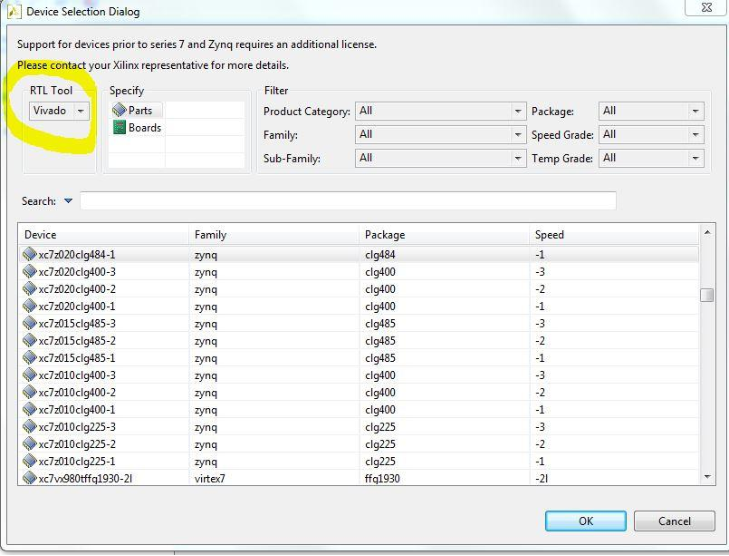
\includegraphics{images/xillybus_wrapper}
\caption{Make sure to select Vivado as the design tool.}
\label{fig:xillybus_wrapper}
\end{figure}

\begin{figure}[!h]
\centering
%\includesvg{images/matrix_vector_sequential}
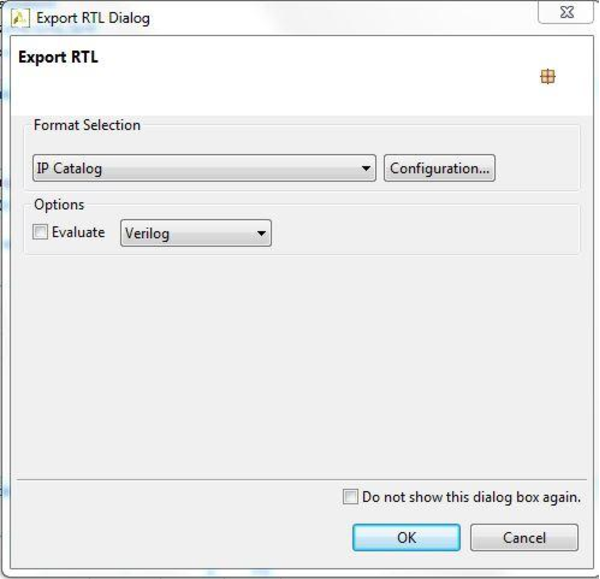
\includegraphics{images/xillybus_settings}
\caption{Required settings for exporting RTL into XIllybus.}
\label{fig:xillybus_settings}
\end{figure}

\section{Report}

Your report should mostly focus on the design of your CORDIC core. For this, I want you to use understand how the precision of the CORDIC core affects the performance and area of your designs. The precision is affected by the number of rotations, and also the bitwidths of the data types, both the data types for the input and output arguments, and the data types of the internal variables. 

You should investigate both of these sources of imprecision by generating a number of different designs. One should plot how the number of rotations affects the performance (throughput/latency) and the area (DSP48s, BRAMS, LUTs, FFs). 

The second source of imprecision is how the number of bits for the fixed point variables that you use. Again, you should investigate how changing the fixed point bits for the variables affects the precision, area, and performance. 

In both cases, you should plot some graphs. Talk about the trends. Give insights into why these trends make sense. Talk about trends or data points that do not make sense.

Some ideas to discuss in your report:
\begin{enumerate}
\item What is the total throughput of your Phase Detector? How does that relate to the individual components (FIR, CORDIC, etc.)? How can you make it better?
\item I am looking for deep insight into the design. Why does the accuracy stop improving after so many iterations? What is the minimal amount of bits required for each variable? Does this depend on the input data? If so, can you characterize the input data to help you restrict the number of required bits? Do different variables require different number of bits?
\item The ultimate goal of the CORDIC is not to use only simple operations, i.e., add and shift. You should not be using divide, multiply, etc. in your CORDIC core.
\item How does the ternary operator \texttt{?} synthesize? Is it useful in this project? 
\end{enumerate}

